%%%%%%%%%%%%%%%%%%%%%%%%%%%%%%%%%%%%%%%%%%%%%%%%%
%%%%%%%  DUNE COMPUTING MODEL. Start of work October2015.    %%%%%%%%%%%%%%%%
%%%%%%%%%%%%%%%%%%%%%%%%%%%%%%%%%%%%%%%%%%%%%%%%%

\documentclass[12pt]{article}

\topmargin=-0.5in
\oddsidemargin=0in
\evensidemargin=0in
\textwidth=6.2in
\textheight=9.25in

\usepackage[dvips]{graphics}
\usepackage[nomargin,inline,marginclue,draft]{fixme}
\usepackage{rotating}
\usepackage{amssymb,amsmath}
\usepackage{graphicx}
\usepackage{cite}
\usepackage{color}
\usepackage[table]{xcolor}
\usepackage{colortbl}
\usepackage{enumerate}

%\usepackage[titletoc]{appendix}

\usepackage{multirow}

%% draftwatermark causes infinite loop on SL6's ancient TeXLive
\usepackage[firstpage]{draftwatermark}
\usepackage{lipsum}
\usepackage{tikz}

\usepackage[T1]{fontenc}
\usepackage[utf8]{inputenc}
%\usepackage[blocks,affil-it]{authblk}

\usepackage{xspace}


\newcommand{\pd}{protoDUNE\xspace}
\newcommand{\filesize}{8\,GB\xspace}

% experimental - for diameter symbol etc
\usepackage{wasysym}

\RequirePackage{lineno}

\bibliographystyle{plain}
\bibliographystyle{unsrt}

\usepackage{graphicx, subfigure}
\usepackage[colorlinks=true,urlcolor=black,linkcolor=black,citecolor=black,bookmarks=true]{hyperref}

% Depth can be adjusted, and 3 may seem excessive, but when set to 2, a lot of interesting detail in TOC is lost.
\setcounter{tocdepth}{3}


\begin{document}

%\linenumbers

\title{The \pd-SP prompt processing system
and its application in Data Quality Monitoring}

\date{\today}

\maketitle

\centerline{The DUNE Collaboration}


\SetWatermarkText{DRAFT}
\SetWatermarkLightness{0.9}
\SetWatermarkScale{3}

\vspace{2cm}

\begin{abstract}

\noindent  The Deep Underground Neutrino Experiment (DUNE) will employ a uniquely
large Liquid Argon Time Projection chamber as the main component of its Far Detector.
It will include four 10kt modules which will include single and dual-phase Liquid Argon
technologies. In order to validate its design an ambitious experimental program (named
''protoDUNE'') has been initiated which includes a beam test of large-scale DUNE prototypes
at CERN in 2018. This presentation concerns itself with the single-phase detector. The volume
of data to be collected in this test will amount to a few petabytes and the sustained rate of
data sent to mass storage will be in the range of a few hundred MB per second. In addition
to careful design of the Data Acquisition, Online Monitoring and Data Handling systems,
the protoDUNE experiment requires substantial Data Quality Monitoring capabilities in
order to ascertain the condition of the detector and its various subsystems. To this end,
a Prompt Processing system has been designed which is complementary to Online Monitoring
and is characterized by lower bandwidth, substantial CPU resources and end-to-end latency
on the scale of a few minutes. We present the design of the ProtoDUNE Prompt Processing
system, the current status of its development and testing and issues related to its interfaces
and deployment.

\end{abstract}


% --- executive summary section ---
\newpage
%\centerline{\textbf{\centerline{\bf{\Large {Executive Summary}}}}} 
%\input{execsum}

%++++++++++++++++++++++++++++++++++++++++
% TOC and lists of tables and figures
%\newpage
%\tableofcontents
%\newpage
%\listoftables
\newpage
%\listoffigures

\newpage


\section{Overview of the protoDUNE-SP experiment}
The \pd program aims to validate various aspects of the DUNE  Liquid Argon Time Projection Chamber (LArTPC)  technology 
before proceeding with the construction of the large-scale principal DUNE detectors at the Sanford Underground Research
Facility \cite{cdrVol1, cdrVol4}. It  is designed to make a series of measurements of the interactions of
charged particles in the Liquid Argon medium.  These measurements will be performed with a dedicated test
beam line  at the CERN SPS accelerator complex which will allow the transport of beam particles from $\sim$0.5 GeV/c
up to 7 GeV/c. The run plan also includes a large number of cosmic ray triggers. The program includes
two separate large LArTPC prototypes, one based on a ``single-phase'' (liquid) technology and
the other based on a ``dual-phase'' (liquid/gaseous) TPC readout technology.
Both detectors are placed in an extension of the CERN North Area Experimental Hall and  scheduled
to take data in 2018. The general layout of the experimental area is shown in Fig.\,\ref{fig:np02np04}, with
the single-phase detector seen as a cubic structure on the right.

Located in the vicinity of the detectors will be enclosures which will house the elements of the local computing infrastructure
(including Data Acquisition, Online Buffer etc). These enclosures are shown schematically as yellow blocks in the
upper-right portion of Fig.\,\ref{fig:np02np04}, and they will have a dedicated 20 Gb/s
network connection over optical fiber to the CERN central storage facilities.

%%%%%%%%%%%%%%%%%%%%%%%%
\begin{figure}[tb]
\centering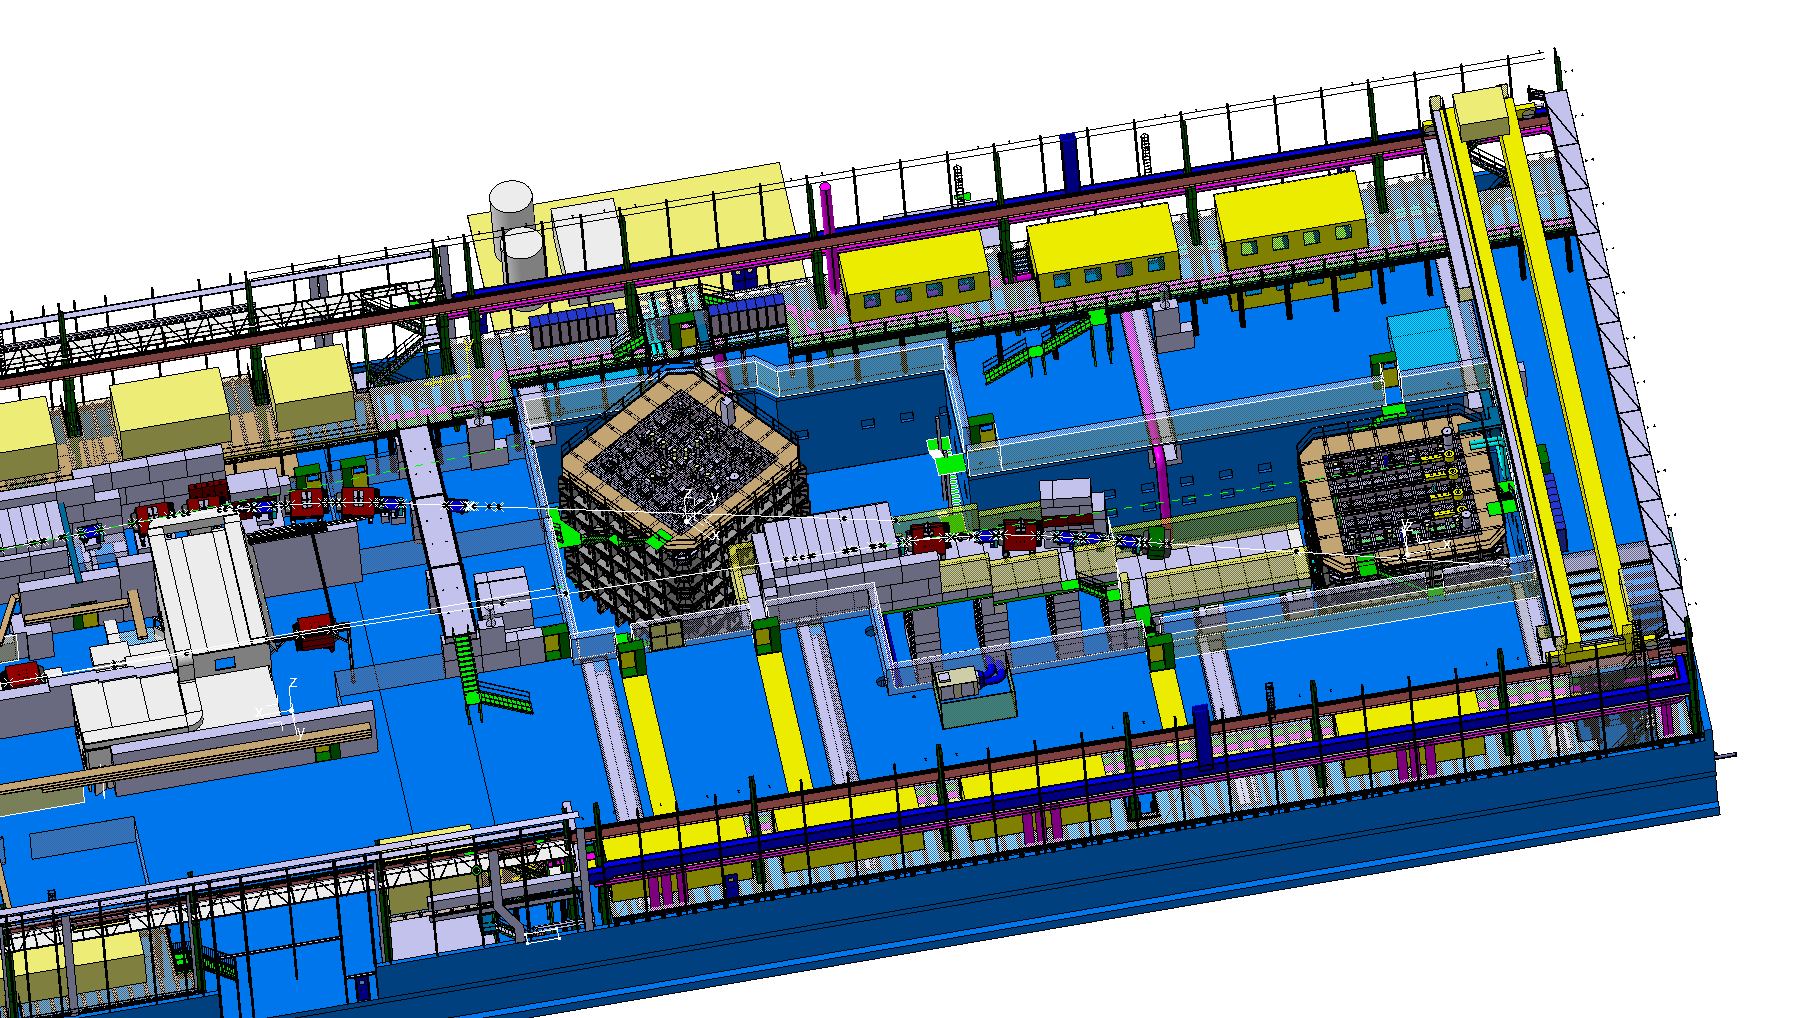
\includegraphics[width=1.0\textwidth]{figures/np02np04.png}
\caption{\label{fig:np02np04}Diagram of the layout of the CERN north area with
  location of the protoDUNE dual phase detector (center) and the single
  phase detector (right). The direction of the particle beam is from left to right.}
\end{figure}




\end{document}


